\documentclass{article}
\usepackage{graphicx} % Required for inserting images

\title{Assignment 1: Wheatstone Bridge with Long-wire
Compensation using a Three-wire Sensor}
\author{Moaaz Mostafa Ibrahim \hspace{20pt} 2400862}
\date{}

\begin{document}
\maketitle

We must prove that this circuit results in the relation $\Delta V = C \cdot \Delta R$, given that $R_1 = R_2 = R_3 = R$ and $\; R_4 = R + \Delta R$.
\begin{figure}[h]
    \centering
    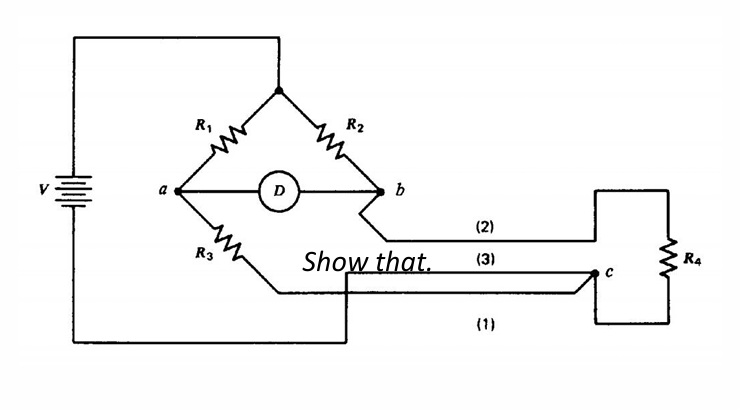
\includegraphics[width=\linewidth]{Media/Bridge.png}
    \caption{Wheatstone Bridge with Long-wire Compensation}
    \label{fig:1}
\end{figure}\\
Let the horizontal lower wire be grounded and denote the resistance of the wires (1), (2), and (3) by $r$.\\
The voltage at $a$ can be evaluated as $V_a = I_s r + \frac{V}{2R + r}\cdot (r + R)$. Similarly, the voltage $V_b = I_s r + \frac{V}{2R + \Delta R + r}\cdot (r + R + \Delta R)$. Therefore: 
$$\Delta V = V\cdot (\frac{R+r}{2R + r} - \frac{R+\Delta R+r}{2R+\Delta R + r}) = V\cdot \frac{\Delta R (-R)}{(2R+r)(2R + \Delta R + r)}$$
Knowing that $R>>\Delta R$, then $2R + r >>\Delta R$. Using this assumption we can simplify the expression for $\Delta V$ as follows.
$$
\Delta V \approx -\Delta R \cdot \frac{VR}{(2R + r)^2} = C \cdot \Delta R
$$

\end{document}
